% Figure: the three-level stratification of the axiom system. Referenced from
% rem:strata. Pure TikZ; the plan table's "three-level containment" figure.

\begin{figure}[tbp]
\centering
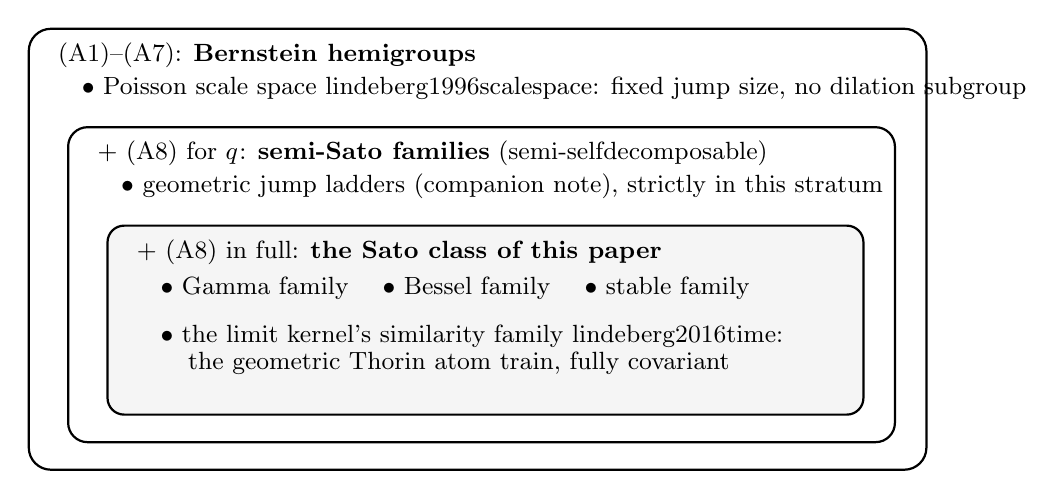
\begin{tikzpicture}[every node/.style={font=\small}, line cap=round]

% three nested rounded boxes
\draw[rounded corners=8pt, thick] (0,0) rectangle (11.4,5.6);
\node[anchor=north west] at (0.25,5.55) {(A1)--(A7): \textbf{Bernstein hemigroups}};
\node[anchor=west] at (0.55,4.85) {$\bullet$ Poisson scale space \sscite{lindeberg1996scalespace}: fixed jump size, no dilation subgroup};
\draw[rounded corners=7pt, thick] (0.5,0.35) rectangle (11.0,4.35);
\node[anchor=north west] at (0.75,4.3) {+ (A8) for $q^{\ZZ}$: \textbf{semi-Sato families} (semi-selfdecomposable)};
\node[anchor=west] at (1.05,3.6) {$\bullet$ geometric jump ladders (companion note), strictly in this stratum};
\draw[rounded corners=6pt, thick, fill=gray!8] (1.0,0.7) rectangle (10.6,3.1);
\node[anchor=north west] at (1.25,3.05) {+ (A8) in full: \textbf{the Sato class of this paper}};
\node[anchor=west] at (1.55,2.3) {$\bullet$ Gamma family \quad $\bullet$ Bessel family \quad $\bullet$ stable family};
\node[anchor=west] at (1.55,1.7) {$\bullet$ the limit kernel's similarity family \sscite{lindeberg2016time}:};
\node[anchor=west] at (1.9,1.35) {the geometric Thorin atom train, fully covariant};

\end{tikzpicture}
\caption{The three-level stratification of Remark~\ref{rem:strata}. The axioms without
covariance admit the Bernstein hemigroups, where the Poisson scale space lives and stays;
covariance under a discrete subgroup $q^{\ZZ}$ cuts out the semi-Sato stratum, whose strict
members are geometric refinements of it; full continuous covariance cuts out the class
characterized in this paper, which contains the similarity family generated by the
time-causal limit kernel's exponent. Containment, not competition: the earlier
constructions occupy strata of one axiom system.}
\label{fig:strata}
\end{figure}
